\documentclass[12pt]{article}
\usepackage{url, graphicx}
\usepackage{geometry}
\usepackage{amsmath}
\usepackage{fancyhdr}
\usepackage{nopageno}
\pagestyle{fancy}

\title{\huge Lecture 4: Recursive Algorithms: Fast Multiplication; Fast Matrix Multiplication}
\author{}
\date{}
\pagestyle{fancy}
\fancyhf{}
\lhead{COMP 251 Winter 2018}
\rhead{Lecture 4}
\lfoot{$15^{th}$ Jan, 2018}
\rfoot{\copyright{}Yutong Yan}

\newcommand{\forceindent}{\leavevmode{\parindent=1em\indent}}
\begin{document}
\maketitle
\section{Multiplication}
\renewcommand{\labelitemii}{$\circ$}
\renewcommand{\labelitemiii}{$\cdot$}
\renewcommand{\labelitemiii}{$\rightarrow$}
\begin{itemize}
\item{Grade School Multiplication}
	\begin{itemize}
	\item Perform $n^2$ multiplications to multiply two n-digit numbers
		\begin{itemize}
		\item Long multiplication has running time $\Omega$($n^2$).
		\end{itemize}
	\end{itemize}
\item Russian Peasant Multiplication\\
	Mult(x, y)\\
	\textbf{If} x = 1 \textbf{then} output y\\
	\textbf{If} x is odd \textbf{then} output y + Mult([{\large $\frac{x}{2}$}],2y)\\
	\textbf{If} x is even \textbf{then} output Mult({\large $\frac{x}{2}$},2y)\\
	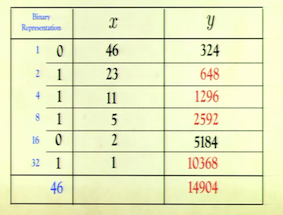
\includegraphics{lecture41}
	\begin{itemize}
	\item This method does work. Base case (x = 1) is verified. The step when x is even also works. The only tricky step is that x is odd when you divide x by 2, you actually divide x by 2 and minus a half, so that you need to add one y back.
	\item How long does it take? \\
	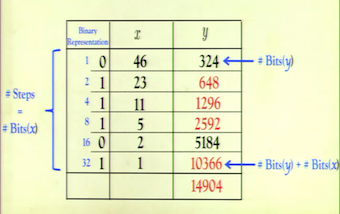
\includegraphics{lecture42}
		\begin{itemize}
		\item There are n iterations, so we add up to n numbers with at most 2n digits each.
		\item Runtime = $O$($n^2$)
		\end{itemize}
	\end{itemize}
\end{itemize}

\section{Divide and Conquer Multiplication}
\renewcommand{\labelitemii}{$\circ$}
\renewcommand{\labelitemiii}{$\cdot$}
\renewcommand{\labelitemiii}{$\rightarrow$}
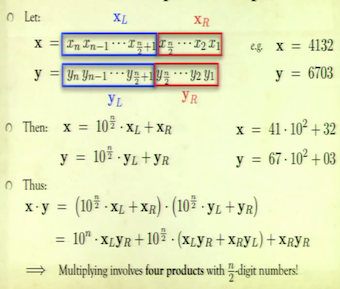
\includegraphics{lecture43}
\begin{itemize}
\item How long does this algorithm take?
	\begin{itemize}
	\item The recursive formula for the running time is:
	
	\hspace*{\fill} {\large $T$(n) = 4 $\cdot$ $T$($\frac{n}{2}$) + $O$(n) } \hspace*{\fill} 
	
	Note: by padding some zeroes in front of the number, we can assume n is a power of 2.
	\item Thus we have a = 4, b = 2, and d = 1.
	\item This is Case 3 of the Master Theorem.
	\item Runtime = $O$($n^{\log_2 4}$) = $O$($n^2$)
	\end{itemize}
\end{itemize}

\section{Gauss's Complex Number Multiplication}
\renewcommand{\labelitemii}{$\circ$}
\renewcommand{\labelitemiii}{$\cdot$}
\renewcommand{\labelitemiii}{$\rightarrow$}
\begin{itemize}
\item Gauss considered the product of complex numbers: 
\begin{center}
 (a + b $\cdot$ $i$) $\cdot$ (c + d $\cdot$ $i$) = ac - bd + (bc + ad) $\cdot$ $i$  
 \end{center}
 \item This seems to require taking \textbf{four products}, but he observed that:
 \begin{center}
 (bc + ad) = (a + b) $\cdot$ (c + d) - ac - bd
\end{center}
\item So we can calculate ac and bd then we only need to perform only one more product to find (bc + ad), namely (a + b) $\cdot$ (c + d).
	\begin{itemize}
	\item Multiplying two complex numbers involves only \textbf{three products}! We got extra addition here, but addition is much cheaper than multiplication when we think about the running time.
	\end{itemize}
\end{itemize}

\section{Application of Gauss's Complex Number Multiplication}
\renewcommand{\labelitemii}{$\circ$}
\renewcommand{\labelitemiii}{$\cdot$}
\renewcommand{\labelitemiii}{$\rightarrow$}
\begin{itemize}
\item We can simply replace \textbf{i} by $10^{\frac{n}{2}}$\\
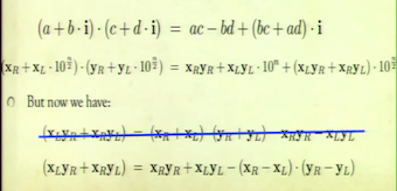
\includegraphics{lecture44}
	\begin{itemize}
	\item Multiplying involves only \textbf{three products} with ${\frac{n}{2}}$ digit numbers!
	\end{itemize}
\item The recursive formula for the running time is: 

	\hspace*{\fill} {\large $T$(n) = 3 $\cdot$ $T$($\frac{n}{2}$) + $O$(n) } \hspace*{\fill} 
	
\item Thus we have a = 3, b = 2, and d = 1.
\item This is Case 3 of the Master Theorem.
\item Runtime = $O$($n^{\log_2 3}$) = $O$($n^{1.59}$)
\item So we can multiply two n-bit numbers using less than $n^2$ operations!
\end{itemize}

\section{Fast Fourier Transforms}
\renewcommand{\labelitemii}{$\circ$}
\renewcommand{\labelitemiii}{$\cdot$}
\renewcommand{\labelitemiii}{$\rightarrow$}
\begin{itemize}
\item We can multiply two n-bit numbers in time $O$(n $\cdot$ $\log{}n$) using a \textbf{Fast Fourier Transform}.
\item More generally, FFTs can be used to multiply two \textbf{polynomial functions}.
	\begin{itemize}
	\item This has a vast number of applications, for example in \textit{image compression} and \textit{signal processing}.
	\item Indeed, it has been described by Strang as "the most important numerical algorithm of our lifetime."
	\end{itemize}
\item We might study FFTs later in the course.
\end{itemize}

\section{Matrix Multiplication}
\renewcommand{\labelitemii}{$\circ$}
\renewcommand{\labelitemiii}{$\cdot$}
\renewcommand{\labelitemiii}{$\rightarrow$}
\begin{itemize}
\item High School Matrix Multiplication\\
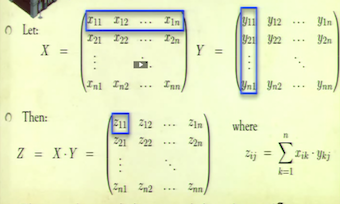
\includegraphics{lecture45}\\
Then we perform n multiplications to calculate each entry of $Z$.
\item Runtime = $\Omega$($n^3$)
\end{itemize}

\section{Divide and Conquer Matrix Multiplication}
\renewcommand{\labelitemii}{$\circ$}
\renewcommand{\labelitemiii}{$\cdot$}
\renewcommand{\labelitemiii}{$\rightarrow$}
\begin{itemize}
\item We can also multiply matrices using \textbf{divide and conquer}.\\
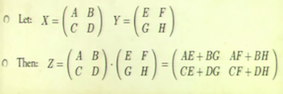
\includegraphics{lecture46}
\item Multiplying involves \textbf{eight products} with $\frac{n}{2}$ $\times$ $\frac{n}{2}$ matrices!
\item The recursive formula for the running time is:
	
	\hspace*{\fill} {\large $T$(n) = 8 $\cdot$ $T$($\frac{n}{2}$) + $O$($n^2$) } \hspace*{\fill} 
	
	\item Thus we have a = 8, b = 2, and d = 2.
	\item This is Case 3 of the Master Theorem.
	\item Runtime = $O$($n^{\log_2 8}$) = $O$($n^3$)
	\item No improvement!
\end{itemize}

\section{An Algebraic Trick for Matrix Multiplication}
\renewcommand{\labelitemii}{$\circ$}
\renewcommand{\labelitemiii}{$\cdot$}
\renewcommand{\labelitemiii}{$\rightarrow$}
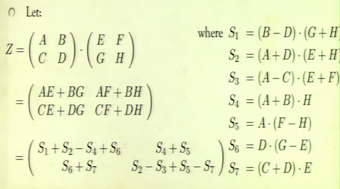
\includegraphics{lecture47}
\begin{itemize}
\item Multiplying involves \textbf{seven products} with $\frac{n}{2}$ $\times$ $\frac{n}{2}$ matrices!\\
Note: Even though we now have 18 additions, the runtime is still dominated by the number of multiplications. Having additions would not hurt.
\item The recursive formula for the running time is:
	
	\hspace*{\fill} {\large $T$(n) = 7 $\cdot$ $T$($\frac{n}{2}$) + $O$($n^2$) }\hspace*{\fill} 
	
	\item Thus we have a = 7, b = 2, and d = 2.
	\item This is Case 3 of the Master Theorem.
	\item Runtime = $O$($n^{\log_2 7}$) = $O$($n^{2.81}$)
\item This divide and conquer matrix multiplication algorithm was designed by Strasser (1969). Since then \underline{faster} algorithms (in theory) have been developed:
	\begin{itemize}
	\item \textbf{Theorem}: There is a matrix multiplication algorithm that runs in time $O$($n^{2.37}$)
	\item \textbf{Open Problem}: Is matrix multiplication $O$($n^{2 + \epsilon}$) time for any constant $\epsilon$ $>$ 0?
	Note: There is no way you can beat this because just to read the matrix x you have to do $x^2$ amount of work to read entries in x simply for y. Getting running time like this seems crazy but possible.
	\end{itemize}
\end{itemize}

\section{Fast Exponentiation}
\renewcommand{\labelitemii}{$\circ$}
\renewcommand{\labelitemiii}{$\cdot$}
\renewcommand{\labelitemiii}{$\rightarrow$}
\begin{itemize}
\item Suppose we want to compute $x^n$
	\begin{itemize}
	\item The slow way $x$ $\cdot$ $x$ $\cdot$ $\cdot$ $\cdot$ $x$ requires n-1 multiplications.
	\item A faster way is to use the fact that $x^n$ = $x^{[\frac{n}{2}]}$ $\cdot$ $x^{[\frac{n}{2}]}$
	\end{itemize}
\item The latter method gives the following \textbf{recursive algorithm}.\\
\\
{\large
\underline{Fast Exponentiation}\\
\textbf{FastExp}(x,n)\\
\textbf{If} n = 1 \textbf{then} output x\\
\textbf{Else} \\
\forceindent \textbf{If} n is even \textbf{then} output \textbf{FastExp}$(x,[\frac{n}{2}])^2$\\
\forceindent \textbf{If} n is odd \textbf{then} output \textbf{x $\cdot$ FastExp}$(x,[\frac{n}{2}])^2$
}
\item The number of multiplications used in Fast Exponentiation satisfies:
\begin{center}
{\large
$T$(n) $\leq$ $T$($[\frac{n}{2}]$) + 2 $\Rightarrow$ $T$(n) = $T$($\frac{n}{2}$) + $O$(1)}
\end{center}
\item Thus we have a = 1, b = 2, and d = 0.
\item This is Case 2 of the Master Theorem.
\item Runtime = $O$($n^0 \cdot log{}n$) = $O$($log{}n$)
\end{itemize}









\end{document}